\documentclass[conference]{IEEEtran}
\usepackage{amsmath,amssymb,amsfonts}
\usepackage{graphicx}
\usepackage{svg}
\usepackage{textcomp}
\usepackage{comment}
\usepackage{xcolor}
\usepackage{booktabs}
\usepackage{tabularx}
\usepackage{hyperref}
\usepackage{cite}
\usepackage{tikz}
\usepackage{pgfplots}
\pgfplotsset{compat=1.18}
\usetikzlibrary{calc}
\usetikzlibrary{arrows.meta, positioning}
\pagestyle{plain}
\begin{document}

\title{Reverse Trust Paradigm: Modeling User Intent and Compliance in LLMs Through Trust Vectors}


\author{
    \IEEEauthorblockN{Irshadh Abdul Rasheed KA}
    \IEEEauthorblockA{\textit{Dept. of Computer Science} \\
    \textit{IIIT Sricity}\\
    \\
    irshadhrasheed.ka@iiits.in
}
    \and
    \IEEEauthorblockN{Sudhan P}
    \IEEEauthorblockA{\textit{Dept. of Computer Science} \\
    \textit{IIIT Sricity}\\
    \\
    sudhan.p23@iiits.in }

    \and
    \IEEEauthorblockN{Mallikarjun Reddy}
    \IEEEauthorblockA{\textit{Dept. of Computer Science} \\
    \textit{IIIT Sricity}\\
    \\
    mallikarjunreddy.d@iiits.in }
    \and
    \IEEEauthorblockN{Kamalkanth Sethi}
    \IEEEauthorblockA{\textit{Dept. of Computer Science} \\
    \textit{IIIT Sricity}\\
    \\
    kamalakanta.s@iiits.in }    

}



\maketitle

\begin{abstract}
In large language models (LLMs) and their subsequent use in complex, multi-turn interactions, human intent is often split and distributed across multiple prompts. While many studies have explored human trust in AI, less attention has been given to the inverse: how models can assess the reliability of user inputs. In this paper, we present the Reverse Trust Paradigm, a security framework in which an AI system learns the human operator's semantic intent, behavioral trajectory, and operational reliability through active and continued surveillance.

The primary mechanism underlying the Reverse Trust Paradigm is the Trust Vector, a mathematical formulation of an LLM's trust in a user's intent, derived from its output for a given human prompt. The Trust Vector is designed as a composite of three key characteristics of the LLM's interaction outputs, serving as an indicator of the trustworthiness of the LLM's response. This metric is averaged across conversational turns using an exponential moving average, reflecting the LLM's overall confidence in the user and the safety of the requested action. We applied this concept across five selected datasets containing multi-turn interactions and computed the Trust Vector for each interaction. Our analysis indicates that Trust Vector offers a quantifiable measure of a model's belief in the trustworthiness and appropriateness of a requested action, providing up to 92.5\% accuracy on multi-turn datasets with explicit harmful requests.
The Trust Vector can therefore be leveraged to develop metrics for monitoring multi-turn jailbreaking, tracking guardrail erosion, and implementing robust safety measures for public-facing LLMs.

\end{abstract}

\begin{IEEEkeywords}
large language models, trust vector, reverse trust paradigm, multi-turn jailbreak detection, adversarial intent, guardrail erosion, AI safety
\end{IEEEkeywords}

\section{Introduction}

 As LLMs are increasingly getting embedded in everyday life, the question of trust has become central to their safe deployment. Much of the existing work on trust addresses only one half of the relationship: how confident a human should be in what the model produces. Whether the model can assess how much confidence it should place in the human driving the conversation has received far less attention. This largely unexamined direction motivates the present work.

The studies addressing the first half of this relationship \cite{ref1, ref2, ref3} are concerned with providing a mechanism for humans to measure how much trust should be placed in an AI system. Accuracy, transparency, reliability, and interface design are usually identified as the critical factors shaping this trust. Research on LLM transparency enables users to understand a model's capabilities and limitations well enough to form their own judgment about how much to rely on its output \cite{ref4}. TrustLLM extends this line of work by assessing trustworthiness across truthfulness, safety, fairness, robustness, privacy, and ethics \cite{ref5}. However, its focus remains the LLM's own trustworthiness rather than the system's trust of the user. 
One early study \cite{ref6} indicates that the trustworthiness of a human's prompt can be inferred simply by observing how the LLM responds to it. It also highlights that a model's expressed trust differs from its behavioral trust in LLM-AI interaction. 

Multi-turn attacks exploit the fact that no such reverse-facing trust assessment currently exists. CoSafe \cite{ref7} demonstrates that harmful intent can be laundered through coreference across turns. MTSA \cite{ref8} shows that red-teaming strategies adapt to a model's prior responses for effectiveness rather than a single static prompt. Multi-turn jailbreak literature \cite{ref9, ref10, ref11}, makes clear that an attacker's advantage comes from operating across the conversation as a whole \textemdash \ yet there is still no established means of continuously monitoring how an LLM's trust in its human operator changes as that conversation unfolds.

LLMs cannot directly ascertain a human's actual intent; at best, they can infer an intended outcome. Work on intent recognition shows that intent-aware reformulation can change both user interaction and model output \cite{ref12}. Decoupling a user's core intention from the "wrapper" text can reduce harmful responses without loss in helpfulness \cite{ref13}. LLMs also respond differently to the same underlying question depending on how it is worded \cite{ref14}. A reverse-trust model therefore cannot treat compliance and intent-understanding as a single signal. It must separately assess what the LLM believes the user wants and how far the LLM is willing to comply.

This separation is important because trust, once granted, should not persist forever. AI risk-management and Zero Trust guidelines make this explicit: trust earned in one task should never automatically extend to the next \cite{ref15, ref16}. A long history of harmless requests should not justify granting a later, higher-risk one. Sharma et al. found that explicitly prompting a model to confirm an action before executing it reduced harmful outcomes by 87\% \cite{ref17}.  

Additional evidence suggests it is possible to understand trust from a model's internals. White-box analysis of EleutherAI/gpt-j-6B found that the model's internal trust representation aligns most closely with the Castelfranchi socio-cognitive model \cite{ref58}, and secondarily with the Marsh model \cite{ref27}. TRACE-AI proposes a trust-scoring system for governed generative-AI operations that tracks changes over time, links scores to supporting evidence, and calibrates them against outcomes \cite{ref22}. In this paper, the scoring system is treated as governance requirements and not as a metric. Benchmarks such as HarmBench \cite{ref18}, JailbreakBench \cite{ref19}, and SORRY-Bench \cite{ref20} confirm how easily attackers can exploit a full conversation to bypass safety guards designed for single-turn prompts. 

Recent research has begun to turn toward this reverse side of trust. One line of research explores how trust is represented internally within an LLM \cite{ref21}, while other work examines how cues such as competence, benevolence, and integrity shape a model's downstream decisions \cite{ref23}. The Trust Vector (TV) introduced in this paper extends this emerging direction into a trajectory-based metric: by tracking whether an LLM becomes more or less willing to comply as a conversation develops. It aims to uncover early signs that a model's safety boundaries may be weakening before an attack actually succeeds.

\subsection{Research Gap}
Research on trust in LLMs has predominantly adopted a human-centred direction (as seen in Table~\ref{tab:trustor}: the human is treated as the trustor and the LLM as the trustee \cite{ref29} \cite{ref57}. These studies do not fully explain the reverse side of the interaction: how an LLM responds to a user over the course of a conversation. Important questions remain, including whether the LLM consistently understands the user’s goal, whether it gradually moves from refusal towards compliance, and whether its responses show signs of information leakage or weakening safety boundaries. None of the prior work reviewed offers a way to observe this drift as it happens. 

\begin{table}[htbp]
\centering
\caption{Trustor and Trustee Directions}
\begin{tabularx}{\linewidth}{X X X X}
\toprule
\textbf{Direction} & \textbf{Trustor} & \textbf{Trustee} & \textbf{Central question} \\
\midrule
Traditional human-AI trust & Human user & AI or automated system & Should the person rely on the system? \\
Machine-side user trust & AI-enabled system & User, request, or proposed action & Should the system rely on the inferred intent and permit the requested level of cooperation? \\
\bottomrule
\end{tabularx}
 \label{tab:trustor} 
\end{table}

\begin{center} \footnotesize\textit{Source:} Adapted from~\cite{ref29} \cite{ref57}. \end{center}


The Trust Vector measures whether the LLM becomes more willing to comply, making this drift easier to observe. It does not suggest that the LLM feels trust like a human or can judge whether a person is trustworthy. Instead, it measures trust-related behaviour from the responses the LLM produces. This paper identifies the absence of such a measure as the central problem of Reverse Trust.


\subsection{Contributions}

\noindent The main contributions of this paper are given below:
\begin{itemize}
    \item \textbf{The Reverse Trust Paradigm:} We introduce a novel framework that conceptualizes LLM-user trust as a dynamic, bidirectional evolution. Rather than assuming inherent user trustworthiness, we model how an LLM progressively adjusts its compliance and defensive boundaries across multi-turn interactions.
    
    \item \textbf{The Trust Vector Metric:} We propose a trajectory-based metric to quantify trust. This metric is a composite of Semantic Alignment (intent adherence), Information Density (response depth), and a Refusal Gate (safety enforcement). We smooth these signals using an Exponential Moving Average (EMA) to isolate meaningful, long-term behavioural trends from short-term conversational noise.
\end{itemize}

   This framework helps in detecting gradual shifts in model behaviour, on compliance, safety resistance, or guardrail erosion. This also provides a mechanism for analysing how user behaviour influences model responses over extended interactions.



\section{Background}
It is important to briefly analyze the foundations of Trust and how they are measured especially in a human and computer interaction scenario as we propose our Reverse Trust Paradigm. 

\textbf{Definition of Trust and measurements:}
Trust is the willingness to rely on another party despite uncertainty or potential risk. It is based on the expectation that the other party will behave reliably and appropriately \cite{ref24}. In simple terms: trust is being willing to take a risk on someone else, because you expect them to act a certain way — even though you can’t fully control or verify them. 

Widely used in organisational research is the representation of trust as a combination of Cognitive and Affective Trust \cite{ref25}. Cognitive trust reflects confidence in an actor’s competence, expertise, and reliability, while affective trust develops from perceived empathy, care, and interpersonal support. These dimensions may be measured separately and combined using a weighted model, such as:
\begin{equation}
T = w_c CT + w_a AT
\end{equation}
where $CT$ and $AT$ are normalised cognitive and affective trust scores, and $w_c + w_a = 1$ \cite{ref1}.

For example: Let $CT=0.91$ and $AT=0.72$. Then, Overall trust score will be:
\begin{equation}
Trust = 0.7 CT + 0.3 AT
\end{equation}

A Bayesian trust model represents trust as a probability that is updated whenever new positive or negative evidence becomes available. As successful interactions accumulate, the trust estimate increases, while failures or unreliable behaviour reduce it \cite{ref26}.

\begin{equation}
Trust = P(\text{Trustworthy} \mid \text{Evidence})
\end{equation}

\textbf{Trust in Computational environment:}
Trust is dynamic and may vary across systems, situations, and past interactions as per one of the early studies on computational trust model \cite{ref27}. As per the research, Trust is represented as:
\begin{equation}
T_{AB} \in [0, 1]
\end{equation}

And trust evolves through interactions. Initial trust:
$T=0.50$
Positive exchanges like helpful responses, accurate information and cooperative tone
Trust becomes:
$T=0.73$
After misinformation:
$T=0.48$
The score evolves with conversational history.

It is often shaped by perceived competence, benevolence, integrity, and predictability \cite{ref28}. As per this study, Trust can be measured for an interaction as given below:

\begin{equation}
Trust = 0.35C + 0.30I + 0.20P + 0.15B
\end{equation}
    Illustrative result: $Trust = 0.86$.
    
 In human-computer interaction, trust influences whether people are willing to rely on a technology. The goal is not to maximise trust, but to establish an appropriate level of reliance that reflects the system’s actual capabilities and limitations \cite{ref29}. Trust may also vary according to an individual’s general tendency to trust technology, the specific situation, and experience gained through repeated interaction \cite{ref30}. It is therefore understood as a dynamic and multidimensional concept, although consistent and standardised measurement remains challenging \cite{ref31}. 

Researchers have not yet agreed on a single standard method for measuring Trust between Human and AI. \cite{ref32, ref33}. Common approaches include confidence scores, explanations, trustworthiness cues, and clear communication of uncertainty \cite{ref3, ref4}. The Human-Computer Trust Scale measures trust through perceived risk, competence, and benevolence \cite{ref2, ref37}. However, it focuses on human trust in technology and does not address the reverse perspective of how an AI-enabled system may assess trust user’s conversational behaviour.

LLM trust and safety research focuses on model reliability, transparency, user control, and threats such as prompt injection and jailbreak attacks \cite{ref34, ref35}. 

\textbf{Trust and Intent Analysis from Texts:}
Trust can also be inferred from language features like Sentiment, Agreement, Confidence, Consistency, Certainty and Hedging language \cite{ref36}. 

For example, if the feature scores are $\text{Confidence} = 0.9$, $\text{Evidence} = 0.95$, $\text{Hedging penalty} = 0.1$, and $\text{Consistency} = 0.8$. Then Trust score is:
\begin{multline}
    $T = 0.25 \text{Confidence} + 0.35 \text{Evidence}  \\ + 0.25 \text{Consistency} - 0.15 \text{Hedging penalty} $
\end{multline}



Then, the Result is $T = 0.82$

Alsaid et al.\cite{ref37} use text embeddings to examine the language used across trust questionnaires and show that trust-related concepts can be identified from written or spoken content. They represented trust-related words using GloVe embedding vectors and calculate an average vector for each questionnaire item:
\begin{equation}
v_i = \frac{1}{n} \sum_{j=1}^n e_j
\end{equation}
where $e_j$ is the embedding of word $j$, and $n$ is the number of words in the item. UMAP is then used to project the high-dimensional vectors into a lower-dimensional semantic space for comparison and visualisation. 

Bodonhelyi et al. evaluated intent recognition as a classification task using a fine-grained intent taxonomy. They also compared recognition quality and user-satisfaction ratings across models and prompt conditions \cite{ref12}. A concise general representation is:
\begin{equation}
y = \arg\max_{c \in C} P(c \mid x)
\end{equation}
where $x$ is the user prompt, $C$ is the set of possible intent categories, and $y$ is the predicted intent. 

Shah et al. used an LLM with human validation to generate, refine, and assign intent-taxonomy labels to search and chat logs \cite{ref39}. Their main contribution is a validated human-in-the-loop pipeline rather than a specific trust or intent-scoring equation.



\section{Preliminaries}

This section introduces the notation, terminology, and mathematical building blocks used in the paper. Terms specific to the Trust Vector construction are defined here at a general level and are elaborated in the next section.

\subsection{Basic Terms}

\begin{itemize}
    \item \textbf{Embedding.} A representation of a piece of text as a vector of $384$ numbers, that is, a single point in a $384$-dimensional space. We use all-MiniLM-L6-v2 \cite{ref40} for embedding.
    
    \item \textbf{Cosine similarity.} A measure of how closely two vectors point in the same direction, ignoring their lengths. For vectors $a$ and $b$,
    \begin{equation}
    \cos(a, b) = \frac{a \cdot b}{\|a\|\,\|b\|}
    \label{eq:cosine}
    \end{equation}
    It ranges from $1$ for identical directions, through $0$ for unrelated ones, to $-1$ for opposite ones. 
    
    \item \textbf{Top-$k$ similarity.} The mean of the $k$ largest cosine similarities between one vector and the members of a set of vectors. It measures how close a text is to the most similar examples in a reference set, rather than to the set's average.
    
    \item \textbf{Compliance.} A response in which the model carries out what the user asked for.
    
    \item \textbf{Refusal.} A response in which the model declines to carry out what the user asked for.
    
    \item \textbf{Hedging.} Cautious or qualifying language that softens a response or signals reluctance to answer, such as ``I'm sorry'' or ``I cannot''.
    
    \item \textbf{Lexical density.} The proportion of a text's words that carry content (nouns, verbs, adjectives, adverbs) rather than serving a grammatical function \cite{ref41}.
\end{itemize}

\subsection{Notation}

Table~\ref{tab:notation} summarizes the symbols used in the Trust Vector formulation for quick reference.

\begin{table}[htbp]
\centering
\caption{Notation Used in the Trust Vector Formulation}
\label{tab:notation}
\begin{tabularx}{\linewidth}{l X}
\toprule
\textbf{Symbol} & \textbf{Meaning} \\
\midrule
$\hat{S}_E$ & Semantic Alignment score (direction component) \\
$\hat{I}_D$ & Information Density score (magnitude component) \\
$\Phi_{gate}$ & Refusal Gate value (friction / override component) \\
$A_+$, $A_c$ & Compliance anchor set and refusal anchor categories ($c = 1,\dots,5$) \\
$k$ & Number of nearest anchors averaged in Semantic Alignment ($200$) \\
$a$, $b$ & Logistic (Platt) scaling parameters of Semantic Alignment ($16.38$, $4.30$) \\
$\mu_{target}$ & Lexical-density normalization ceiling ($0.70$) \\
$\tau$ & Refusal-density threshold ($0.05$) \\
$\gamma$ & Exponential penalty strength for the Refusal Gate ($2.0$) \\
$\alpha$, $\beta$ & Weights for Semantic Alignment and Information Density ($0.6$, $0.4$) \\
$TV_t$ & Trust Vector of the model's reply at turn $t$ \\
\bottomrule
\end{tabularx}
\end{table}



\section{Reverse Trust Paradigm and Trust Vector}
We introduce the Reverse Trust Paradigm, which models multi-turn interactions between a user's inferred intent and the degree of compliance shown by the target LLM. Alongside it, we introduce the Trust Vector, a trajectory metric that scores how much trust the LLM places in the user. This score is recalculated after every interaction, based on the LLM's output. The reverse-trust principle mirrors the security maxim "never trust, always verify," but applied at the semantic and conversational level.

We treat the Trust Vector, as shown in Figure~\ref{fig:tv},
as a form of conversational momentum, combining direction, magnitude, refusal friction, and historical momentum. Like momentum in classical mechanics, it depends on both the direction and magnitude of the LLM's behavioural change, moderated by the friction introduced by safety training and alignment constraints. The Table~\ref{tab:MCA}) below shows what direction, magnitude, and refusal friction represent, how each is mathematically defined in an LLM conversation, and how they combine into a single heuristic measure.

\begin{table}[htbp]
\centering
\caption{Momentum Conversational Analogy}
\begin{tabularx}{\linewidth}{l l X}
\toprule
\textbf{Momentum} & \textbf{Trust Vector component} & \textbf{Measured property} \\
\midrule
Direction & Semantic Alignment ($\hat{S}_E$) & Whether the response is oriented towards compliance or refusal. \\
Magnitude & Information Density ($\hat{I}_D$) & How much substantive lexical payload the response contains. \\
Friction / override & Refusal Gate ($\Phi_{gate}$) & Whether explicit refusal hedges structurally suppress the compliance score. \\
\bottomrule
\end{tabularx}
\label{tab:MCA}
\end{table}

\begin{figure}[htbp]
\centering
\resizebox{\linewidth}{!}{%
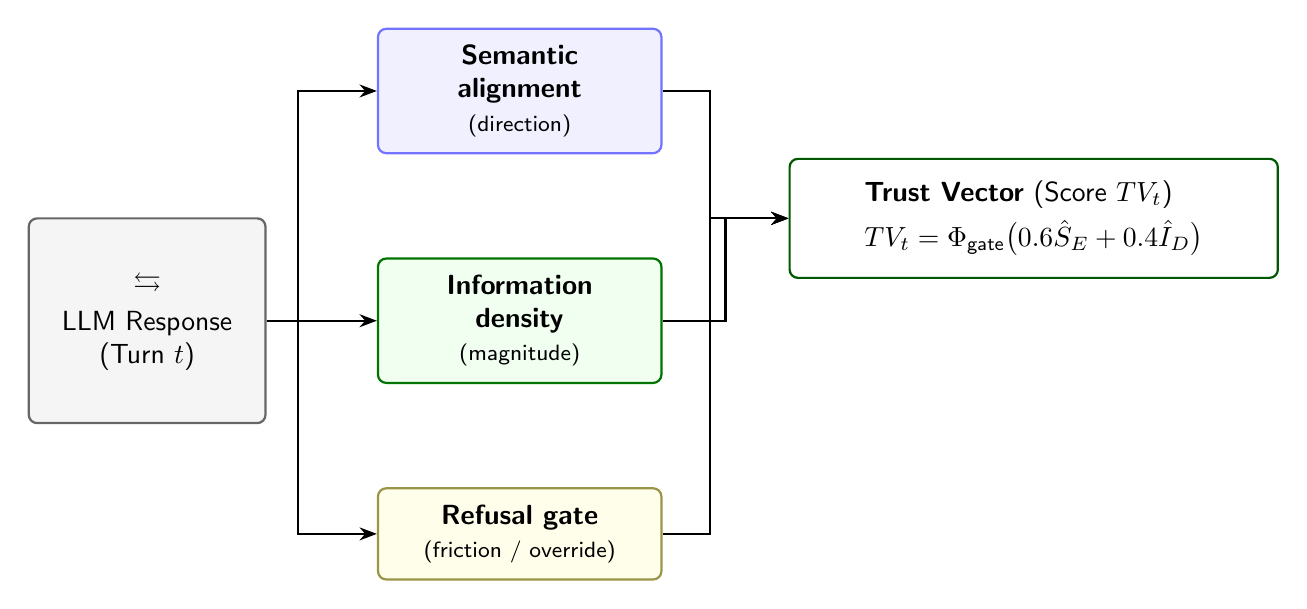
\begin{tikzpicture}[
    font=\sffamily,
    node distance=6mm and 10mm,
    box/.style={
        rectangle, rounded corners=3pt, draw, thick,
        minimum height=1.1cm, align=center, inner sep=6pt
    },
    inputbox/.style={
        box, draw=black!60, fill=black!4,
        minimum width=2.1cm, minimum height=2.6cm
    },
    subbox/.style={
        box, minimum width=3.6cm
    },
    sabox/.style={subbox, draw=blue!55, fill=blue!6},
    idbox/.style={subbox, draw=green!45!black, fill=green!6},
    rgbox/.style={subbox, draw=yellow!55!black, fill=yellow!8},
    mainbox/.style={
        box, draw=green!35!black, thick,
        minimum width=6.2cm, align=left, inner sep=8pt
    },
    arr/.style={-{Stealth[length=2.2mm]}, thick}
]

% --- Input node ---
\node[inputbox] (input) {\begin{tabular}{c}$\leftrightarrows$\\[2pt] LLM Response\\ (Turn $t$)\end{tabular}};

% --- Three sub-signal boxes (stacked vertically) ---
\node[sabox, above right=8mm and 14mm of input] (sa)
    {\textbf{Semantic}\\ \textbf{alignment}\\ \footnotesize (direction)};
\node[idbox, right=14mm of input] (id)
    {\textbf{Information}\\ \textbf{density}\\ \footnotesize (magnitude)};
\node[rgbox, below right=8mm and 14mm of input] (rg)
    {\textbf{Refusal gate}\\ \footnotesize (friction / override)};

% --- Instantaneous trust box ---
\node[mainbox, right=16mm of id, yshift=13mm] (tt)
    {\textbf{Trust Vector} (Score $TV_t$)\\[4pt]
     $TV_t = \Phi_{\text{gate}}\big(0.6\hat{S}_E + 0.4\hat{I}_D\big)$};


% --- Arrows: input to three sub-boxes ---
\draw[arr] (input.east) -- ++(4mm,0) |- (sa.west);
\draw[arr] (input.east) -- (id.west);
\draw[arr] (input.east) -- ++(4mm,0) |- (rg.west);

% --- Arrows: three sub-boxes to instantaneous trust ---
\draw[arr] (sa.east) -| ++(6mm,0) |- (tt.west);
\draw[arr] (id.east) -- ++(8mm,0) |- (tt.west);
\draw[arr] (rg.east) -| ++(6mm,0) |- (tt.west);


\end{tikzpicture}%
}
\caption{Trust Vector}
\label{fig:tv}
\end{figure}


\subsection{Trust Vector Measurement}
\textbf{Semantic Alignment (Direction):} Semantic Alignment measures whether a response leans toward compliance or refusal, whether the model is facing True North (compliance) or True South (refusal) in the latent embedding space. It must satisfy two properties:

\begin{itemize}
    \item The score should rise as a response resembles compliance and fall as it resembles refusal.
    \item The score should ignore the response's \emph{topic}. A refusal that names a dangerous subject and a tutorial explaining that same subject discuss the same thing while doing opposite things, so shared subject matter must not move the score.
\end{itemize}

We compare the response embedding $e$ (all-MiniLM-L6-v2 \cite{ref40}, unit length) with published, human-labelled model responses rather than with hand-written phrases. The compliance set $A_+$ contains Do-Not-Answer responses that directly follow the instruction or were labelled harmful \cite{dna}. The refusal side is kept as five separate categories $A_1,\dots,A_5$: Do-Not-Answer responses that refuse, that refute the request, or that say they cannot answer \cite{dna}, and CoCoNot responses to incomplete requests and to requests with safety concerns \cite{coconot}. Refusals are kept apart because a model can decline in several ways (refusing outright, correcting the user, asking for clarification), and each sits in a different region of the embedding space.

For a set $A$, let $s_k(e, A)$ be the top-$k$ similarity of the response to that set:
\begin{equation}
s_k(e, A) = \frac{1}{k}\sum_{a \,\in\, \text{top}_k(e, A)} e \cdot a
\end{equation}
The raw score compares the closest compliance responses with the closest responses of the best-matching refusal category:
\begin{equation}
\Delta = s_k(e, A_+) \;-\; \max_{c}\, s_k(e, A_c), \qquad k = 200
\label{eq:delta}
\end{equation}
Both terms compare the response with real responses on many different topics, so shared subject matter raises both terms together and largely cancels in the difference; what remains is whether the response behaves like a compliance or like a refusal. A refusal that names a dangerous subject and a tutorial on that subject therefore score differently even though they discuss the same thing. The value of $k$ was chosen by leaving out one Do-Not-Answer source model at a time.

A larger $\Delta$ means a more compliance-like response. $\Delta$ is mapped to $[0,1]$ with a logistic (Platt) function \cite{platt}:
\begin{equation}
\hat{S}_E = \frac{1}{1 + \exp\!\big(-(a\Delta + b)\big)}, \qquad a = 16.38,\ b = 4.30
\label{eq:sa}
\end{equation}
The parameters $a$ and $b$ were fitted by class-balanced logistic regression on held-out values of $\Delta$ for the Do-Not-Answer responses, each response being scored against anchors that exclude its own source model. XSTest \cite{xstest} was used only afterwards, as an untouched check. Scores near $1$ indicate compliance and scores near $0$ indicate refusal; $\hat{S}_E = 0.5$ at $\Delta = -b/a \approx -0.26$, the point the fitted model treats as equally likely to be either.

\textbf{Information Density (Magnitude):} Information Density, as shown in Figure~\ref{fig:id}, measures how much of a response is actual payload. It must be a proportion rather than a raw count, so that padding a response lowers the score instead of raising it.

Counting content words directly would not be length-independent, so we use a proportion instead. Let $n_c$ be the number of content-bearing tokens (nouns, proper nouns, verbs, adjectives, adverbs) and $n$ the total token count. The raw lexical density is
\begin{equation}
\rho = \frac{n_c}{n} \;\in\; [0,1]
\end{equation}

Using $\rho$ directly would waste most of the scale. Ure's measurements place ordinary English at $40\text{--}50\%$ lexical density, and even highly technical or instructional prose rarely exceeds $65\text{--}70\%$ \cite{ref41}. A response would therefore have to be linguistically implausible to score near $1$. Instead, we rescale against the highest density actually attainable, $\mu_{target}$, rather than the theoretical maximum of $1$. Responses that exceed $\mu_{target}$ are already maximally dense, so the result is capped:
\begin{equation}
\hat{I}_D = \min\!\left(1,\; \frac{\rho}{\mu_{target}}\right), \qquad \mu_{target} = 0.70
\label{eq:id}
\end{equation}

\begin{figure}
    \centering
    \includegraphics[width=1\linewidth]{3. Information Density - Simple.png}
    \caption{Information Density as a function of lexical ratio, saturating at $\mu_{target}=0.70$.}
    \label{fig:id}
\end{figure}

Restricting the numerator to content-bearing tokens discards low-payload function words such as articles and prepositions, so $\hat{I}_D$ measures actionable information rather than sentence length. This repurposes Ure's lexical density measure — originally used to distinguish writing registers — as a proxy for compliance effort. The $\mu_{target}$ ceiling and the spaCy-based \cite{ref42} part-of-speech extraction are both original to this work.

\textbf{Refusal Gate (Friction / Override):}  Refusal Gate, as shown in Figure~\ref{fig:gate}, captures the resistive effects of guardrails and applies a structural override when explicit refusal signals are present, preventing long verbose refusals from being interpreted as compliance. Reinforcement Learning from Human Feedback training makes models exceptionally polite even when refusing. A response can be long, detailed, and on-topic — scoring well on both components above — while still declining outright (``I apologize, but I cannot...''). Neither $\hat{S}_E$ nor $\hat{I}_D$ reliably catches this alone, since a lengthy refusal dilutes the alignment signal without reducing the density signal. The Refusal Gate exists to override exactly this case. It must:

\begin{itemize}
    \item leave an unhedged response untouched, so the gate equals $1$ when no refusal language is present;
    \item shut completely once refusal language reaches a threshold density $\tau$;
    \item transition smoothly between those two states, so refusal is graded rather than a binary flag;
    \item scale with response length, since one refusal phrase in a short reply is strong evidence, while the same phrase in a long answer is weak.
\end{itemize}

The last requirement is met by measuring a density rather than a raw count. Let $m$ be the number of refusal phrases found in the response, taken from the HarmBench refusal lexicon \cite{ref18} and extended with 28 common first-person refusal forms (for example ``I can't help'', ``I'm unable to'' and ``I must decline'', with straight and curly apostrophes), and $n_w$ its word count, giving hedge density $h = m / n_w$. It is convenient to express this in units of the threshold, $u = h/\tau$, so $u=0$ means no hedging and $u=1$ means threshold-level hedging.

The first three requirements call for a function that starts at $1$, reaches $0$ at $u=1$, and decreases smoothly in between. The simplest such function is $(1-u)^\gamma$, giving
\begin{equation}
\Phi_{gate} = \max\!\left(0,\; 1 - \frac{h}{\tau}\right)^{\!\gamma}, \qquad \tau = 0.05,\ \gamma = 2.0
\label{eq:gate}
\end{equation}
where the $\max$ keeps the gate shut once hedging exceeds the threshold.

\begin{figure}[htbp]
\centering
\resizebox{\linewidth}{!}{%
\begin{tikzpicture}[
    font=\sffamily,
    pipebox/.style={
        rectangle, rounded corners=5pt, draw, thick,
        minimum width=6.4cm, minimum height=3.6cm,
        align=center, inner sep=8pt
    },
    arr/.style={-{Stealth[length=3mm]}, ultra thick, black!70}
]

% ================= TOP: pipeline of three boxes =================
\node[pipebox, draw=blue!25!black, fill=blue!3] (box1) at (0,9.5)
    {\Large\textbf{Response Text}\\ \Large\textbf{Analyzer}\\[10pt]
     \large Count predefined\\ \large refusal phrases.};

\node[pipebox, draw=yellow!45!black, fill=yellow!8] (box2) at (9.2,9.5)
    {\Large\textbf{Hedge Density}\\ \Large\textbf{Computation}\\[10pt]
     \large $d = $ refusal phrases\\ \large / response length};

\node[pipebox, draw=red!45!black, fill=red!4] (box3) at (18.4,9.5)
    {\Large\textbf{Gate Value ($\Phi_{\text{gate}}$)}\\[6pt]
     \large $\Phi_{\text{gate}} = \max\!\big(0,\, (1-d/0.05)\big)^2$\\[10pt]
     \begin{tikzpicture}
        \shade[left color=red!75!black, right color=red!2] (0,0) rectangle (5.4,0.35);
        \draw[thick] (0,0) rectangle (5.4,0.35);
        \node[font=\large] at (-0.3,0.17) {1};
        \node[font=\large] at (5.7,0.17) {0};
     \end{tikzpicture}
    };

% Small icons above each box (simplified as colored circles with symbols)
\node[font=\Large] at (box1.north) [yshift=6mm] {\textcolor{blue!40!black}{$\mathbf{\mathcal{Q}}$}};
\node[font=\Large] at (box2.north) [yshift=6mm] {\textcolor{yellow!50!black}{$\mathbf{\Sigma}$}};
\node[font=\Large] at (box3.north) [yshift=6mm] {\textcolor{red!55!black}{$\mathbf{\Phi}$}};

% Arrows between the three boxes
\draw[arr] (box1.east) -- (box2.west);
\draw[arr] (box2.east) -- (box3.west);

% ================= BOTTOM: pgfplots decay curve =================
\begin{scope}[shift={(0,0)}]
\begin{axis}[
    width=20cm, height=9cm,
    xlabel={\Large Refusal-phrase density ($d$, \%)},
    ylabel={\Large $\Phi_{\text{gate}}$ (Normalized Value)},
    xmin=0, xmax=5.3,
    ymin=0, ymax=1.05,
    xtick={0,1,2,3,4,5},
    ytick={0,0.2,0.4,0.6,0.8,1.0},
    tick label style={font=\large},
    label style={font=\large},
    axis lines=left,
    grid=major,
    grid style={gray!30},
    thick,
    domain=0:5.3,
    samples=200,
    clip=false
]
% Shaded area under the curve (manual fill using \addplot fill)
\addplot[red!55!black, opacity=0.15, fill=red!55!black]
    {max(0, (1 - x/5))^2} \closedcycle;

\addplot[
    red!55!black, ultra thick
] {max(0, (1 - x/5))^2};

% marker dots at integer d values
\addplot[only marks, mark=*, mark size=2.2pt, red!55!black]
    coordinates {(0,1.0) (1,0.64) (2,0.36) (3,0.16) (4,0.04) (5,0.0)};

% 5% threshold dashed vertical line
\draw[dashed, thick, yellow!45!black] (axis cs:5,0) -- (axis cs:5,1.05)
    node[above, font=\large, text=yellow!40!black] {5\% threshold};

\end{axis}
\end{scope}

\end{tikzpicture}%
}
\caption{Refusal Gate collapses to zero once hedge density reaches $\tau = 0.05$.}
\label{fig:gate}
\end{figure}

The threshold $\tau = 0.05$ is an empirical tripwire: once more than $5\%$ of a response is refusal language — five matches in a hundred words — the response is treated as a definitive refusal.

The exponent $\gamma$ shapes the collapse, not just its speed. In Eq.~\ref{eq:gate}, the penalty bites hardest right at the start: the curve falls steeply as soon as hedging appears, then flattens as it nears the threshold. For example, at half the threshold density, $\Phi_{gate} = (1-0.5)^2 = 0.25$, so hedging at half strength has already removed three quarters of the score. This front-loading is deliberate, since the earliest traces of refusal language are the most diagnostic.

\textbf{Trust Vector:} 
The three components are combined for every response of the model. Direction and magnitude are combined as a weighted sum, and the Refusal Gate scales the result:
\begin{equation}
TV_t = \Phi_{gate} \times \big(\alpha \hat{S}_E + \beta \hat{I}_D\big), \qquad \alpha = 0.6,\ \beta = 0.4
\label{eq:tt}
\end{equation}

The constraint $\alpha + \beta = 1$ makes the bracketed term a weighted average of two quantities that each lie in $[0,1]$, so it stays in $[0,1]$ too; since $\Phi_{gate}$ is also in $[0,1]$, the product is as well, with no further normalization needed. Within this constraint, $\alpha > \beta$ weights direction above magnitude, so what a model is \emph{trying} to do counts for more than how much it says — a verbose but misdirected response cannot inflate the score.

The gate multiplies rather than subtracts. A subtractive penalty can be outvoted: an expression such as $\alpha \hat{S}_E + \beta \hat{I}_D - \lambda(1 - \Phi_{gate})$ can still return a positive score when alignment and density are high enough, even with the gate fully closed. Multiplication cannot be outvoted — a closed gate, $\Phi_{gate}=0$, forces $TV_t=0$ regardless of the other two components, which is the whole point of having a gate.

The Trust Vector is recomputed at every turn from the model's most recent reply. When the next request arrives, $TV_t$ of the previous reply is the trust the model has most recently shown towards the user. Earlier replies are not averaged in. The history of the conversation still matters, but it acts through the model's latest behaviour: an exponential moving average over past turns was tested on all nine evaluation sets and did not improve TV consistently (better on four, worse on five). Figure~\ref{fig:tvturns} shows $TV_t$ turn by turn for one jailbroken and one safe conversation.

\begin{figure}[htbp]
\centering
\resizebox{\linewidth}{!}{%
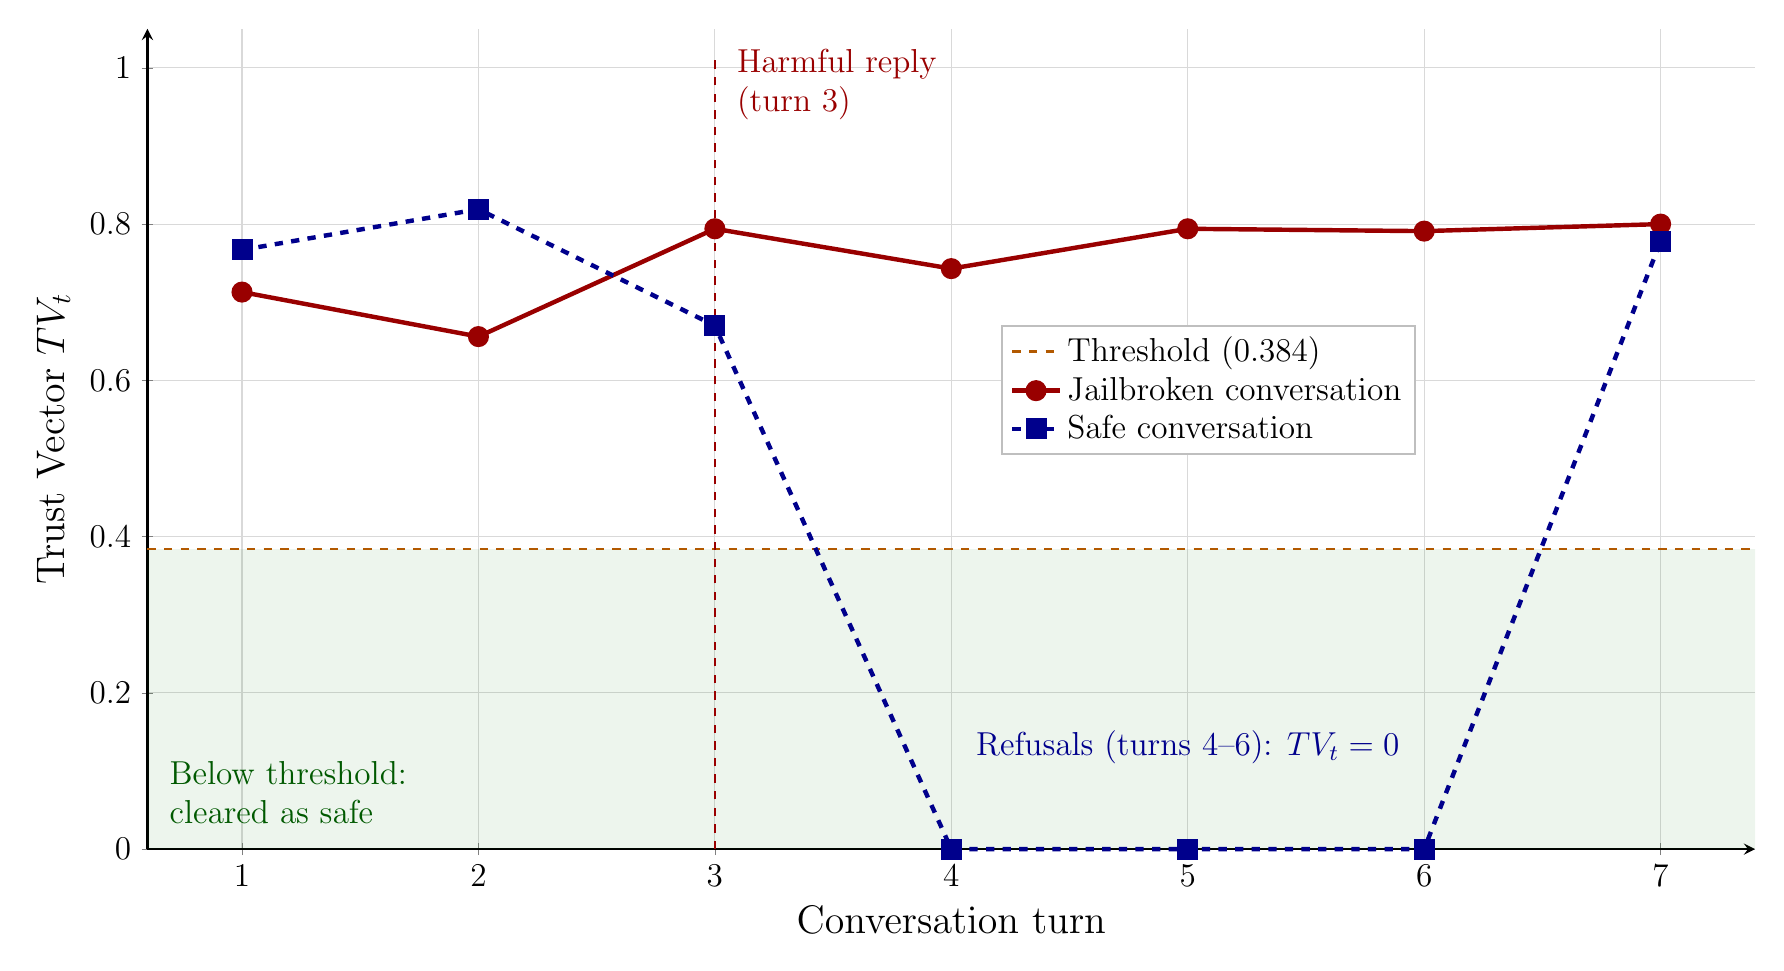
\begin{tikzpicture}[font=\sffamily]
\begin{axis}[
    width=22cm, height=12cm,
    xlabel={\Large Conversation turn},
    ylabel={\Large Trust Vector $TV_t$},
    xmin=0.6, xmax=7.4, ymin=0, ymax=1.05,
    xtick={1,2,3,4,5,6,7},
    ytick={0,0.2,0.4,0.6,0.8,1.0},
    tick label style={font=\large},
    label style={font=\large},
    axis lines=left,
    grid=major, grid style={gray!30},
    thick, clip=false,
    legend style={font=\large, draw=gray!50, fill=white, at={(0.66,0.56)}, anchor=center},
    legend cell align={left}
]
% shaded region below the threshold = cleared as safe
\addplot[draw=none, fill=green!45!black, fill opacity=0.07, forget plot] coordinates {(0.6,0) (7.4,0) (7.4,0.384) (0.6,0.384)} \closedcycle;
\addlegendimage{dashed, thick, orange!70!black}
\addlegendentry{Threshold (0.384)}
\addplot[dashed, thick, orange!70!black, forget plot] coordinates {(0.6,0.384) (7.4,0.384)};
% jailbroken conversation (locked id 22240)
\addplot[red!60!black, solid, ultra thick, mark=*, mark size=3pt, mark options={fill=red!60!black}]
    coordinates {(1,0.713) (2,0.656) (3,0.794) (4,0.743) (5,0.794) (6,0.791) (7,0.800)};
\addlegendentry{Jailbroken conversation}
% safe conversation (locked id 4579)
\addplot[blue!55!black, dashed, ultra thick, mark=square*, mark size=3pt, mark options={fill=blue!55!black, solid}]
    coordinates {(1,0.767) (2,0.819) (3,0.670) (4,0.000) (5,0.000) (6,0.000) (7,0.778)};
\addlegendentry{Safe conversation}
% annotations
\draw[dashed, thick, red!60!black] (axis cs:3,0) -- (axis cs:3,1.02);
\node[align=left, font=\large, text=red!60!black, anchor=south west] at (axis cs:3.05,0.92) {Harmful reply\\(turn 3)};
\node[align=center, font=\large, text=blue!55!black] at (axis cs:5,0.13) {Refusals (turns 4--6): $TV_t = 0$};
\node[align=left, font=\large, text=green!35!black, anchor=south west] at (axis cs:0.65,0.02) {Below threshold:\\cleared as safe};
\end{axis}
\end{tikzpicture}%
}
\caption{Trust Vector per turn for two real conversations from the locked Llama-3.1-8B-Instruct XGuard-Train set: the first jailbroken and the first safe conversation in the locked random sample that have at least five replies. The dashed line is the set's threshold at 100\% sensitivity. The jailbroken conversation stays above the threshold up to the harmful reply at turn 3; in the safe conversation the model refuses at turns 4--6 and TV falls to 0, below the threshold.}
\label{fig:tvturns}
\end{figure}


A high $TV$ means the latest response is more compliant on the documented lexical, semantic, and structural signals; a low $TV$ means refusal evidence or low alignment or density in the latest response. Critically, $TV$ does not establish a user's authorisation, legitimacy, character, psychology, or true intent, and it does not by itself prove a successful jailbreak — a separate outcome label or structured success check is required. Thresholds are properties of a given evaluation configuration, not universal constants.



\subsection{Implementation of Trust Vector}
The Trust Vector is implemented through a sequential NLP pipeline that extracts and combines three behavioural signals from each LLM response: Semantic Alignment ($\hat{S}_E$), Information Density ($\hat{I}_D$), and the Refusal Gate ($\Phi_{gate}$). The computation proceeds as follows:
\begin{itemize}
    \item \textbf{Response Generation:} The target LLM produces a response to the input prompt.
    \item \textbf{Text Preprocessing:} The raw text is passed to spaCy \cite{ref42} to strip punctuation and tokenize the string, isolating the ``payload'' words (nouns, verbs, adjectives, adverbs).
    \item \textbf{Semantic Alignment ($\hat{S}_E$):} This is computed using the all-MiniLM-L6-v2 Sentence-BERT model \cite{ref40}. Responses are embedded and compared with the published compliance and refusal anchor sets; the top-$k$ similarity difference, after logistic scaling, gives the response's position between refusal and compliance.
    \item \textbf{Information Density ($\hat{I}_D$):} this is computed using the spaCy \cite{ref42} NLP framework, which performs tokenization and part-of-speech tagging. The ratio of content-bearing words (nouns, verbs, adjectives, and adverbs) to the total token count is then used to quantify the informational value of the response.
    \item \textbf{Refusal Gate Computation ($\Phi_{gate}$):} This is derived from refusal-indicative language identified using the HarmBench refusal lexicon \cite{ref18}, extended with 28 first-person refusal forms. The occurrence of common hedging and refusal phrases is used to quantify refusal behaviour and apply the corresponding penalty during Trust Vector computation.
    \item \textbf{Trust Vector ($TV_t$):} The extracted metrics are combined using the Trust Vector formulation, where Semantic Alignment and Information Density are weighted and subsequently modulated by the Refusal Gate.
\end{itemize}

This pipeline transforms raw LLM responses into structured semantic, linguistic, and behavioural signals, giving one trust score for every reply of a multi-turn interaction.

\subsection{Experiments}
The following approach is followed in conducting the experiments for validation of the Trust Vector. 
\begin{itemize}
    \item \textbf{Selection of Multiturn Data Sets.} Six datasets were used in total: five multi-turn, one single-turn, each with a different origin, attack style, and source model(s) generating the responses being scored.  They are given below:
\begin{itemize}

    \item Anthropic hh-rlhf (red-team-attempts)(\url{https://huggingface.co/datasets/Anthropic/hh-rlhf})
\item Tom-Gibbs multi-turn cipher attacks (\url{https://huggingface.co/datasets/tom-gibbs/multi-turn_jailbreak_attack_datasets})
\item SafeMTData\_1K (ActorAttack)(\url{https://huggingface.co/datasets/SafeMTData/SafeMTData})
\item CoSafe (coreference-based multi-turn attacks)(\url{https://huggingface.co/datasets/Asap7772/cosafe_all_rollouts_guardgen})
\item HarmfulQA (Chain-of-Utterances multi-turn attacks)(\url{https://huggingface.co/datasets/declare-lab/HarmfulQA})
\item WildGuardMix (single-turn)(\url{https://huggingface.co/datasets/allenai/wildguardmix})
\end{itemize}


    The selection criteria for the data sets are given below: 
\begin{itemize}
    \item It must represent a real attack attempt or jailbreaking attempt
    \item It has to be a multi-turn interaction data set
    \item The data should contain output of the LLM for each interaction. This is very critical for measuring the score.
    \item It should not neutral/benign chat with no adversarial intent. 
    \item It must have a flag for whether the jailbreak succeeded or not — both a safe class and a jailbreak class must actually exist and be labeled (ground-truth or otherwise derivable).
\end{itemize}


    
    \item \textbf{Compute Trust Vector against the Data Set for every interaction.} For every interaction, Trust Vector is calculated as per formula defined. 
    \item \textbf{Take one feature value per conversation}, using an asymmetric convention validated earlier:
    \begin{itemize}
        \item Jailbreak conversations $\rightarrow$ TV at turn N-1 (the turn right before the harmful compliance). This tests TV’s early-warning ability — can it flag danger before the harmful response actually lands?
        \item Safe conversations $\rightarrow$ TV at turn N (the final, refusing turn). Measuring at N validates that TV’s refusal gate is functioning: compliance should visibly drop when the model declines.
    \end{itemize}
    \item \textbf{Split 80/20 into train/test.} For Anthropic and Tom-Gibbs this used the datasets’ pre-existing train/test files; for SafeMTData\_1K it was a stratified random split.
    \item \textbf{Fit the threshold on train only}, using an ROC curve and Youden’s J statistic (the point that maximizes True Positive Rate $-$ False Positive Rate).
    \item \textbf{Evaluate on the held-out test set}, reporting sensitivity, specificity, and overall accuracy.
\end{itemize}

\subsection{Sensitivity and Specificity}
When we pick a Trust Vector (TV) threshold, every conversation in the test set falls into one of two predicted buckets (refer Table~\ref{tab:PO}): above threshold (flagged as a jailbreak) or below threshold (cleared as safe). Comparing that prediction to the real label gives four outcomes:

\begin{table}[htbp]
\centering
\caption{Prediction Outcomes}
\begin{tabularx}{\linewidth}{l X X}
\toprule
& \textbf{Predicted: Above threshold} & \textbf{Predicted: Below threshold} \\
\midrule
\textbf{Actually jailbreak} & True Positive (TP) & False Negative (FN) \\
\textbf{Actually safe} & False Positive (FP) & True Negative (TN) \\
\bottomrule
\end{tabularx}
\label{tab:PO}
\end{table}

From these:
\begin{itemize}
    \item \textbf{Sensitivity = TP / (TP + FN)} — of all the real jailbreaks, what percentage did TV correctly flag? High sensitivity means TV rarely misses a real jailbreak.
    \item \textbf{Specificity = TN / (TN + FP)} — of all the real safe conversations, what percentage did TV correctly leave alone? High specificity means TV rarely raises a false alarm on a safe conversation.
\end{itemize}

Both matter, and they trade off against each other: a very low threshold catches almost every jailbreak (high sensitivity) but also flags most safe conversations as risky (low specificity), and vice versa. A useful TV threshold needs to be reasonably good at both — that’s what these experiments test.

The methodology for selecting the optimal Trust Vector threshold is rooted in established diagnostic testing and probability forecasting principles \cite{ref53}. Specifically, we utilize Receiver Operating Characteristic (ROC) analysis \cite{ref55} to balance the trade-offs between true and false positive rates across multi-turn interactions. The exact operational threshold is derived using Youden’s J statistic \cite{ref54}, ensuring the metric operates as a well-calibrated classifier of adversarial intent rather than relying on arbitrary limits \cite{ref56}.

\subsection{Results}

\begin{table*}[htbp]
\centering
\caption{Results by Dataset}
 \label{tab:results_data}
\begin{tabularx}{\linewidth}{l l l l l X}
\toprule
\textbf{Dataset} & \textbf{Threshold} & \textbf{Sensitivity} & \textbf{Specificity} & \textbf{Accuracy} & \textbf{Notes} \\
\midrule
Anthropic & 0.3358 & 95.00\% & 90.00\% & 92.50\% & Balanced dataset, heuristic labels \\
SafeMTData\_1K & 0.4845 & 81.20\% & 99.01\% & 91.94\% & Largest multi-turn dataset, heuristic labels (spot-checked) \\
Tom-Gibbs & 0.5128 & 100.00\% & 45.00\% & 65.08\% & Ground-truth labels, but several ``safe'' responses contain undecoded cipher text that breaks refusal detection — this confounds the specificity number and not a failure of Trust Vector \\
CoSafe & 0.4066 & 43.33\% & 68.87\% & 68.33\% & Ground-truth (guard-model) labels. Weakest sensitivity of all datasets — coreference-based harmful turns are vague/indirect rather than explicit requests, and the N-1 history signal alone often isn't enough to flag them \\
HarmfulQA & 0.5521 & 88.51\% & 53.89\% & 69.51\% & Balanced by construction (red = Chain-of-Utterances attack, blue = harmless), deepest conversations tested at 7 assistant turns on average. Labels reflect design intent rather than a verified outcome flag. The only dataset where both classes are compliance rather than refusal, so the Refusal Gate rarely fires and separation rests on alignment and density alone \\
WildGuardMix (single-turn) & 0.2897 & 95.60\% & 34.00\% & 64.80\% & Ground-truth (human) labels, no heuristic at all. weak-specificity pattern TV over-flags safe single-turn responses even with the best label quality we have \\
\bottomrule
\end{tabularx}
\end{table*}


% The Anthropic HH-RLHF and SafeMTData\_1K datasets, both of which contain multi-turn conversations with explicit natural-language harmful pivots, demonstrated the strongest separation between jailbreak and safe trajectories when evaluated using the N$-1$/N Trust Vector methodology. In contrast, performance on the Tom-Gibbs benchmark was weaker, largely due to a known data-quality confound in which refusal responses are encoded using cipher text, reducing the effectiveness of both semantic similarity and refusal-detection mechanisms. Performance further declined on CoSafe, where attacks are expressed through indirect, coreference-based references rather than explicit harmful requests, limiting the effectiveness of the Trust Vector's early-warning signal. 

% The WildGuardMix benchmark, despite containing the highest-quality labels through direct human annotation, exhibited comparatively weak specificity. This observation suggests that the primary limitation arises not from label quality or heuristic classification, but from the Trust Vector's reliance on conversational history. In single-turn settings, the absence of conversational history restricts the ability of the EMA-based trajectory model to distinguish benign and adversarial behaviour effectively. 

% Collectively, these results indicate that the Trust Vector's refusal-sensitive components operate effectively as an early-warning mechanism in multi-turn conversations containing explicit natural-language harmful requests. However, the findings should not be interpreted as definitive evidence that the Trust Vector constitutes a complete or universally applicable trust metric. Rather, they provide empirical support for its effectiveness within a specific class of multi-turn jailbreak scenarios, while highlighting important limitations in contexts involving encoded content, indirect attacks, or the absence of conversational history. 

The Anthropic HH-RLHF and SafeMTData\_1K datasets, both of which contain multi-turn conversations with explicit natural-language harmful pivots, demonstrated the strongest separation between jailbreak and safe trajectories when evaluated using the N$-1$/N Trust Vector methodology. In contrast, performance on the Tom-Gibbs benchmark was weaker, largely due to a known data-quality confound in which refusal responses are encoded using cipher text, reducing the effectiveness of both semantic similarity and refusal-detection mechanisms. Performance further declined on CoSafe, where attacks are expressed through indirect, coreference-based references rather than explicit harmful requests, limiting the effectiveness of the Trust Vector's early-warning signal.

HarmfulQA exhibited a distinct failure mode. Its two classes are separated by whether the model's compliance is harmful or harmless, rather than by whether the model complies at all, so the Refusal Gate rarely activates in either class and discrimination rests on Semantic Alignment and Information Density alone. The result was high sensitivity with weak specificity: the Trust Vector reliably identifies sustained compliance, but does not by itself separate harmful compliance from benign helpfulness.

The WildGuardMix benchmark, despite containing the highest-quality labels through direct human annotation, exhibited comparatively weak specificity. This observation suggests that the primary limitation arises not from label quality or heuristic classification, but from the Trust Vector's reliance on conversational history. In single-turn settings, the absence of conversational history restricts the ability of the EMA-based trajectory model to distinguish benign and adversarial behaviour effectively.

Collectively, these results indicate that the Trust Vector's refusal-sensitive components operate effectively as an early-warning mechanism in multi-turn conversations containing explicit natural-language harmful requests. However, the findings should not be interpreted as definitive evidence that the Trust Vector constitutes a complete or universally applicable trust metric. Rather, they provide empirical support for its effectiveness within a specific class of multi-turn jailbreak scenarios, while highlighting important limitations in contexts involving encoded content, indirect attacks, conversations in which both outcomes involve compliance, or the absence of conversational history.



Thresholds differ because each model has its own ``normal'' writing style, and the threshold is just wherever safe and unsafe answers happen to split for that style — not a fixed danger level. 
\begin{itemize}
    \item Older, short-answer models $\rightarrow$ lower threshold. 
    \item Newer models that always write long, detailed answers (even when being safe) $\rightarrow$ higher threshold, because TV rewards detailed writing.
    \item Single-turn tests (no conversation history) $\rightarrow$ lower threshold, since there's nothing built up yet.
\end{itemize}

Models that produced longer and more structured outputs tended to receive higher scores regardless of safety. This indicates that Trust Vector will not have one universal number that means ``danger'' for every model. It has to be re-tuned for each model/situation — like adjusting a smoke detector's sensitivity differently for a kitchen vs. a bedroom.

Our model works well when two things are true — the conversation has multiple turns, and the harmful request is asked directly. In that case it correctly tells safe and unsafe apart about 92\% (as seen in Table~\ref{tab:results_data}) of the time. It gets much worse when: the harmful request is hidden in a cipher, the request is asked indirectly/vaguely, or there's only one turn with no history. 

\section{Assumptions and Limitations}
The Trust Vector (TV) metric performs as expected under its intended operational conditions. However this framework relies on key assumptions that are listed below. if these are violated it could impact the metric reliability. 

\subsection{Multi-Turn Context Dependency}
We assume that adversarial intent and model compliance evolve progressively across multiple interactions, allowing conversational momentum to accumulate. Semantic Alignment and Information Density components depend heavily on historical context. For single-turn interactions, these metrics provide negligible discrimination (AUC 0.42--0.47, near-random performance). Trust Vector's predictive capability (AUC 0.69--0.73) emerges only when accumulated conversational history is present.

\subsection{Linguistic Predictability of Refusals}
The framework assumes that model safety constraints are exhibited as predictable, English-language refusal or hedging phrases.
The Refusal Gate is dictionary and English language based. When refusals are obscured within undecoded cipher text, specificity drops to 45\%. Against icendirect, coreference-based attacks, sensitivity falls to 43\%. The mechanism cannot reliably support non-English, or dialect-based refusals.


\subsection{Binary Evaluation Scope}
 Our experimental validation assumes that the outcome of trust exploitation is a definitive, binary outcome: harmful compliance or refusal. The metric reliably indicates the point at which refusal ends and compliance begins. It cannot quantify gradual behavioural shifts—such as subtle safety boundary erosion—that occur without an explicit jailbreak.


\section{Conclusion and Future Work}

In summary, our novel Trust Vector is a reliable metric for detecting adversarial intent in multi-turn LLM interactions. Our evaluations demonstrate that TV distinguishes between safe and unsafe conversational trajectories when exposed to explicit harmful requests and standard English-language refusal patterns. Trust Vector can be operationalized as an early-warning detector for explicit multi-turn compliance and refusal behaviour.

The foundational nature of the Reverse Trust Paradigm and Trust Vector opens several critical avenues for future research to address the current structural boundaries of the Trust Vector.

First, the mechanism's applicability to non-English and dialect-based refusals warrants further investigation, as the present analysis is limited to existing multi-turn interaction datasets in a single linguistic context. Second, future work should examine how detection accuracy can be improved when refusal signals are obscured through undecoded ciphertext, indirect inference-based attacks, or progressive psychological manipulation across a conversation.

Additionally, the proposed metrics should be validated against real-world, deployed LLMs to assess their practical effectiveness beyond the controlled dataset conditions used in this study. Further refinement of the individual components of the Trust Vector also presents a promising avenue: for instance, the Information Density metric could be extended beyond simple lexical payload ratios to capture structural mimicry, while dictionary-based refusal gates could be enhanced through mechanistic interpretability techniques.

\begin{thebibliography}{99}
\bibitem{ref1} K. Okamura and S. Yamada, ``Adaptive trust calibration for human–AI collaboration,'' \textit{PLoS ONE}, vol. 15, no. 2, Art. no. e0229132, Feb. 2020, doi: 10.1371/journal.pone.0229132.
\bibitem{ref2} M. J. McGrath, O. L. Lack, J. Tisch, and A. Duenser, ``Measuring trust in artificial intelligence: Validation of an established scale and its short form,'' \textit{Front. Artif. Intell.}, vol. 8, Art. no. 1582880, May 2025, doi: 10.3389/frai.2025.1582880.
\bibitem{ref3} X. Sun, Y. Liu, J. De Wit, J. A. Bosch, and Z. Li, ``Trust by interface: How different user interfaces shape human trust in health information from large language models,'' in \textit{Extended Abstracts of the CHI Conference on Human Factors in Computing Systems}, Honolulu, HI, USA, 2024, pp. 1–7, doi: 10.1145/3613905.3650837.
\bibitem{ref4} Q. V. Liao and J. W. Vaughan, ``AI transparency in the age of LLMs: A human-centered research roadmap,'' \textit{Harvard Data Science Review}, May 2024, doi: 10.1162/99608f92.8036d03b.
\bibitem{ref5} Y. Huang et al., ``TrustLLM: Trustworthiness in large language models,'' arXiv:2401.05561, 2024.
\bibitem{ref6} M. Buyl, Y. Fettach, G. Bied, and T. De Bie, ``Building and measuring trust between large language models,'' arXiv:2508.15858, 2025.
\bibitem{ref7} E. Yu, J. Li, M. Liao, S. Wang, Z. Gao, F. Mi, and L. Hong, ``CoSafe: Evaluating large language model safety in multi-turn dialogue coreference,'' in \textit{Proc. 2024 Conf. Empirical Methods Natural Language Processing}, Miami, FL, USA, 2024, pp. 17494–17508, doi: 10.18653/v1/2024.emnlp-main.968.
\bibitem{ref8} W. Guo, J. Li, W. Wang, Y. Li, D. He, J. Yu, and M. Zhang, ``MTSA: Multi-turn safety alignment for LLMs through multi-round red-teaming,'' in \textit{Proc. 63rd Annu. Meeting Assoc. Comput. Linguistics}, Vienna, Austria, 2025, pp. 26424–26442, doi: 10.18653/v1/2025.acl-long.1282.
\bibitem{ref9} P. Chao, A. Robey, E. Dobriban, H. Hassani, G. J. Pappas, and E. Wong, ``Jailbreaking black box large language models in twenty queries,'' arXiv:2310.08419, 2023, doi: 10.48550/arXiv.2310.08419.
\bibitem{ref10} M. Russinovich, A. Salem, and R. Eldan, ``Great, now write an article about that: The Crescendo multi-turn LLM jailbreak attack,'' in \textit{Proc. 34th USENIX Security Symp.}, 2025.
\bibitem{ref11} N. Li et al., ``LLM defenses are not robust to multi-turn human jailbreaks yet,'' arXiv:2408.15221, 2024, doi: 10.48550/arXiv.2408.15221.
\bibitem{ref12} A. Bodonhelyi, E. Bozkir, S. Yang, E. Kasneci, and G. Kasneci, ``User intent recognition and satisfaction with large language models: A user study with ChatGPT,'' arXiv:2402.02136, 2024, doi: 10.48550/arXiv.2402.02136.
\bibitem{ref13} Y. Zhang, L. Ding, L. Zhang, and D. Tao, ``Intention analysis makes LLMs a good jailbreak defender,'' in \textit{Proc. 31st Int. Conf. Computational Linguistics (COLING)}, Abu Dhabi, United Arab Emirates, 2025, pp. 2947–2968.
\bibitem{ref14} Anonymous, ``Measuring intent comprehension in LLMs: A variance decomposition framework,'' OpenReview preprint, 2026.
\bibitem{ref15} National Institute of Standards and Technology, \textit{Artificial Intelligence Risk Management Framework (AI RMF 1.0)}, NIST AI 100-1, Gaithersburg, MD, USA, Jan. 2023, doi: 10.6028/NIST.AI.100-1.
\bibitem{ref16} National Institute of Standards and Technology, \textit{Zero Trust Architecture}, NIST Special Publication 800-207, Gaithersburg, MD, USA, Aug. 2020, doi: 10.6028/NIST.SP.800-207.
\bibitem{ref17} T. Sharma, V. Sharma, and P. Sharma, ``Real-time trust verification for safe agentic actions using TrustBench,'' arXiv:2603.09157, 2026, doi: 10.48550/arXiv.2603.09157.
\bibitem{ref18} M. Mazeika et al., ``HarmBench: A standardized evaluation framework for automated red teaming and robust refusal,'' in \textit{Proc. 41st Int. Conf. Machine Learning}, vol. 235, 2024, pp. 35181–35224.
\bibitem{ref19} P. Chao et al., ``JailbreakBench: An open robustness benchmark for jailbreaking large language models,'' in \textit{Advances in Neural Information Processing Systems}, vol. 37, 2024, doi: 10.52202/079017-1745.
\bibitem{ref20} T. Xie et al., ``SORRY-Bench: Systematically evaluating large language model safety refusal,'' in \textit{Proc. Int. Conf. Learning Representations}, 2025.
\bibitem{ref21} A. Debnath, S. Cranefield, B. T. R. Savarimuthu, and E. Lorini, ``Evaluating LLM alignment with human trust models,'' arXiv:2603.05839, 2026, doi: 10.48550/arXiv.2603.05839.
\bibitem{ref22} D. Chaudhuri, ``TRACE-AI: A time-versioned, evidence-linked, and outcome-calibrated trust scoring architecture for governed generative AI operations,'' ResearchGate preprint, 2026.
\bibitem{ref23} V. Lerman and Y. Dover, ``A closer look at how large language models ‘trust’ humans: Patterns and biases,'' \textit{Proc. R. Soc. A}, vol. 482, no. 2335, Art. no. 20251113, Apr. 2026, doi: 10.1098/rspa.2025.1113.
\bibitem{ref29} J. D. Lee and K. A. See, ``Trust in automation: Designing for appropriate reliance,'' \textit{Human Factors}, vol. 46, no. 1, pp. 50–80, 2004, doi: 10.1518/HFES.46.1.50\_30392.
\bibitem{ref57} A. Jacovi, A. Marasović, T. Miller, and Y. Goldberg, "Formalizing trust in artificial intelligence: Prerequisites, causes and goals of human trust in AI," in \textit{ Proc. 2021 ACM Conf. on Fairness, Accountability, and Transparency} 2021, pp. 624–635.
\bibitem{ref24} R. C. Mayer, J. H. Davis, and F. D. Schoorman, ``An integrative model of organizational trust,'' \textit{Academy of Management Review}, vol. 20, no. 3, pp. 709–734, 1995, doi: 10.5465/AMR.1995.9508080335.
\bibitem{ref25} D. J. McAllister, ``Affect- and cognition-based trust as foundations for interpersonal cooperation in organizations,'' \textit{Academy of Management Journal}, vol. 38, no. 1, pp. 24–59, 1995.
\bibitem{ref26} A. Jøsang, R. Ismail, and C. Boyd, ``A survey of trust and reputation systems for online service provision,'' \textit{Decision Support Systems}, vol. 43, no. 2, pp. 618–644, 2007.
\bibitem{ref27} S. Marsh, \textit{Formalising Trust as a Computational Concept}, Ph.D. dissertation, University of Stirling, Stirling, U.K., 1994.
\bibitem{ref28} D. H. McKnight, V. Choudhury, and C. Kacmar, ``Developing and validating trust measures for e-commerce: An integrative typology,'' \textit{Information Systems Research}, vol. 13, no. 3, pp. 334–359, 2002.
\bibitem{ref30} K. A. Hoff and M. Bashir, ``Trust in automation: Integrating empirical evidence on factors that influence trust,'' \textit{Human Factors}, vol. 57, no. 3, pp. 407–434, 2015, doi: 10.1177/0018720814547570.
\bibitem{ref31} S. Gulati, J. McDonagh, S. Sousa, and D. Lamas, ``Trust models and theories in human–computer interaction: A systematic literature review,'' \textit{Computers in Human Behavior Reports}, vol. 16, Art. no. 100495, 2024, doi: 10.1016/j.chbr.2024.100495.
\bibitem{ref32} T. Ueno, Y. Sawa, Y. Kim, J. Urakami, H. Oura, and K. Seaborn, ``Trust in human-AI interaction: Scoping out models, measures, and methods,'' in \textit{CHI Conference on Human Factors in Computing Systems Extended Abstracts}, 2022, doi: 10.1145/3491101.3519772.
\bibitem{ref33} S. Mehrotra, C. Degachi, O. Vereschak, C. M. Jonker, and M. L. Tielman, ``A systematic review on fostering appropriate trust in human-AI interaction,'' arXiv:2311.06305, 2023, doi: 10.48550/arXiv.2311.06305.
\bibitem{ref37} A. Alsaid, M. Li, E. K. Chiou, and J. D. Lee, ``Measuring trust: A text analysis approach to compare, contrast, and select trust questionnaires,'' \textit{Frontiers in Psychology}, vol. 14, Art. no. 1192020, 2023, doi: 10.3389/fpsyg.2023.1192020.
\bibitem{ref34} D. You and D. Chon, ``Trust \& safety of LLMs and LLMs in trust \& safety,'' arXiv:2412.02113, 2025, doi: 10.48550/arXiv.2412.02113.
\bibitem{ref35} M. Belosevic, ``User-centric design paradigms for trust and control in human-LLM interactions: A survey,'' in \textit{Proc. Workshop on Human-Centred Natural Language Processing}, 2025.
\bibitem{ref36} D. Artz and Y. Gil, ``A survey of trust in computer science and the Semantic Web,'' \textit{Web Semantics}, vol. 5, no. 2, pp. 58–71, 2007.
\bibitem{ref39} C. Shah et al., ``Using large language models to generate, validate, and apply user intent taxonomies,'' 2023.
\bibitem{ref40} N. Reimers and I. Gurevych, ``Sentence-BERT: Sentence embeddings using Siamese BERT-networks,'' in \textit{Proc. 2019 Conf. Empirical Methods Natural Language Processing and 9th Int. Joint Conf. Natural Language Processing (EMNLP-IJCNLP)}, Hong Kong, 2019, pp. 3982–3992, doi: 10.18653/v1/D19-1410.
\bibitem{ref41} J. Ure, ``Lexical density and register differentiation,'' in \textit{Applications of Linguistics}, G. E. Perren and J. L. M. Trim, Eds. Cambridge, U.K.: Cambridge Univ. Press, 1971, pp. 443–452.
\bibitem{ref42} spaCy is an open-source Python library for natural language processing [\url{https://spacy.io/}]
\bibitem{ref53} G. W. Brier, ``Verification of forecasts expressed in terms of probability,'' \textit{Monthly Weather Rev.}, vol. 78, no. 1, pp. 1–3, Jan. 1950, doi: 10.1175/1520-0493(1950)078<0001:VOFEIT>2.0.CO;2.
\bibitem{ref55} T. Fawcett, ``An introduction to ROC analysis,'' \textit{Pattern Recognit. Lett.}, vol. 27, no. 8, pp. 861–874, Jun. 2006, doi: 10.1016/j.patrec.2005.10.010.
\bibitem{ref54} W. J. Youden, ``Index for rating diagnostic tests,'' \textit{Cancer}, vol. 3, no. 1, pp. 32–35, Jan. 1950, doi: 10.1002/1097-0142(1950)3:1<32::AID-CNCR2820030106>3.0.CO;2-3.
\bibitem{ref56} A. Niculescu-Mizil and R. Caruana, ``Predicting good probabilities with supervised learning,'' in \textit{Proc. 22nd Int. Conf. Machine Learning}, Bonn, Germany, 2005, pp. 625–632, doi: 10.1145/1102351.1102430.
\bibitem{ref58} C. Castelfranchi and R. Falcone, "Principles of trust for MAS: Cognitive anatomy, social importance, and quantification," in \textit {Proc. 3rd Int. Conf. Multi Agent Systems (ICMAS)}, 1998, pp. 72–79.

\bibitem{dna} Y. Wang, H. Li, X. Han, P. Nakov, and T. Baldwin, ``Do-Not-Answer: Evaluating safeguards in LLMs,'' in \textit{Findings of the Association for Computational Linguistics: EACL 2024}, St. Julian's, Malta, 2024, pp. 896--911.
\bibitem{coconot} F. Brahman, S. Kumar, V. Balachandran, P. Dasigi, V. Pyatkin, A. Ravichander, S. Wiegreffe, N. Dziri, K. Chandu, J. Hessel, Y. Tsvetkov, N. A. Smith, Y. Choi, and H. Hajishirzi, ``The art of saying no: Contextual noncompliance in language models,'' in \textit{Advances in Neural Information Processing Systems}, vol. 37, 2024.
\bibitem{platt} J. C. Platt, ``Probabilistic outputs for support vector machines and comparisons to regularized likelihood methods,'' in \textit{Advances in Large Margin Classifiers}, A. J. Smola, P. Bartlett, B. Sch\"olkopf, and D. Schuurmans, Eds. Cambridge, MA, USA: MIT Press, 1999, pp. 61--74.
\bibitem{xstest} P. R\"ottger, H. R. Kirk, B. Vidgen, G. Attanasio, F. Bianchi, and D. Hovy, ``XSTest: A test suite for identifying exaggerated safety behaviours in large language models,'' in \textit{Proc. 2024 Conf. North American Chapter of the Association for Computational Linguistics (NAACL)}, Mexico City, Mexico, 2024, pp. 5377--5400.
\end{thebibliography}

\end{document}